%%%%%%%%%%%%%%%%%%%%%%%%%%%%%%%%%%%%%%%%%%%%%%%%%%%%%%%%%%%%%%%%%%%%%%%%
%                                                                      %
%     File: Thesis_Versat.tex                                          %
%     Tex Master: Thesis.tex                                           %
%                                                                      %
%     Author: Andre C. Marta                                           %
%     Last modified :  2 Jul 2015                                      %
%                                                                      %
%%%%%%%%%%%%%%%%%%%%%%%%%%%%%%%%%%%%%%%%%%%%%%%%%%%%%%%%%%%%%%%%%%%%%%%%

\chapter{HDL Simulators}
\label{chapter:simulators}

As mentioned before, HDL simulators play a fundamental role during the different
phases of circuit development, and there are multiple simulation tools that can
be used. However, despite all these tools having more or less the same purpose
(provide a way to validate the circuit being tested), they do not work in the
same way.

Typically, before testing a circuit, a test bench is created. The test bench is
a program, written in a HDL or in a programming language (like SystemC, for
example), that comprises three modules~\cite{tan:vhstas}: stimuli generator,
golden response generator and response analyser, as shown in
Figure~\ref{fig:tb}. The stimuli generator module is responsible for generating
the signals needed to make the circuit work properly. On the other hand, the
golden response generator computes the expected circuit response, based on the
inputs generated by the stimuli generator. Finally, the response analyzer
compares the circuit output signals with the ones generated by the golden
response generator. During simulation, if both signs are equal, it means that
the circuit is working as intended.

\begin{figure}[!htb]
	\centering
	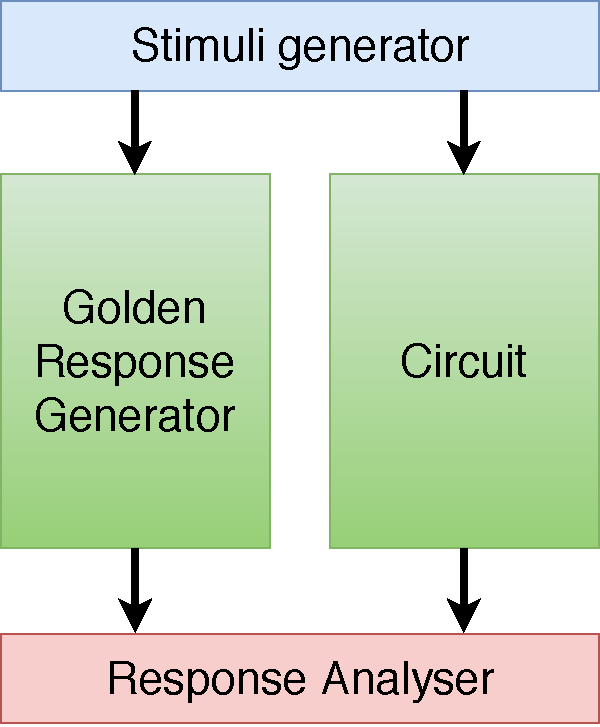
\includegraphics[width=0.42\textwidth]{Figures/Testbench.pdf}
	\caption{Test bench diagram.}
	\label{fig:tb}
\end{figure}

The results provided by the test-bench might depend on the chosen
simulator. This happens because all the simulators work in different ways: while
some focus on obtaining the most complete results (including simulation
timings), sacrificing the speed of the simulations, others do the opposite. In
this perspective, the simulators can be divided into two main categories~\cite{tan:vhstas,palnitkar:verilog}: event-driven or cycle-accurate.

\section{Event-Driven Simulators}
\label{section:event}

The first category of simulators are the event-driven
ones~\cite{tan:vhstas,gunes:survey,palnitkar:verilog}. This simulators work by
taking events sequentially, propagating them through the circuit until it
reaches a steady state.

The events are generated each time that a circuit input is changed, being stored
in a queue, ordered chronologically to allow the correct execution of the
events. When an event is evaluated, only the circuit nodes that have their input
changed by that event are evaluated. After evaluation, the event is removed from
the queue, with new events resultant from the output changes being added. This
means that the same element might be evaluated multiple times during the same
time step due to the feedback from some signals.

It's important to mention that during the simulation process there's a timer
that is used to keep track of the events timings. This leads to one of the main
advantages of event-driven simulation, which is the accurate simulation results,
with detailed timing information, allowing the identification of timing problems
in the tested circuit.

Despite this important advantage, this type of simulation also brings some
disadvantages, mainly related with its speed. Due to their complex algorithms
used for event scheduling and timing evaluation, event-driven simulators are
slow. While for relatively small circuits this might not be a significant
problem, for large circuits this is an important disadvantage, because their
increased complexity will increase significantly the simulation duration.

This type of simulators can be divided into 2 main categories: software or
hardware based, each one with different subcategories. These categories are
analysed in the following subsections.

\subsection{Software-based Simulators}
\label{subsection:software}

The software-based simulators are the most common type of simulators, including
simulators like the Cadence NCSim~\cite{cadence:ncsim}, the Synopsys
VCS~\cite{synopsys:vcs}, the Mentor Graphics ModelSim~\cite{mentor:modelsim} or
the Icarus Verilog~\cite{icarus:verilog}. Usually, they run on a general purpose
computer, being divided into three categories, according to their algorithms:
compiled-code, interpreter and gate level.

An interpreter software simulator reads the HDL code to simulate and interprets
it, translating the original code to a set of instructions accepted by the
simulator program. This translation process occurs during runtime and implies
the creation of data structures to store the data taken from the HDL file, that
will be used afterwards to create the simulation. This simulators are somewhat
inefficient, due to the resultant overhead of the code translation. This
typically results in the execution of a considerable number of instructions per
element evaluation, of which only a few perform logic model evaluation~\cite{lewis:compiled}.

On the other hand, a compiled-code simulator works by transforming the HDL
circuit description, including its testbench, into an equivalent C code (or some
similar programming language). The generated code is then compiled by a generic
complier (like gcc, for example), resulting in an executable file, that will the
be executed to run the simulation. This type of simulators are more efficient
than the interpreter ones, since they eliminate the overhead of traversing the
network data structures~\cite{lewis:compiled}. The most used simulators, like
Cadence NCSim, Synopsys VCS or Icarus Verilog belong to this category of
simulators.

Although the gate level simulators are either of the interpreted or
compiled-code type, they differ from the simulators referred in those
categories~\cite{tan:vhstas}. This happens because, while those simulators have
full Verilog compliance (supporting also gate level simulations), the gate level
simulators just support a small subset of Verilog.

RTL simulation is the most used method for circuit verification due to its
reasonable accuracy~\cite{sousa:reconfigurable}. However, in the last few years
there has been a rising trend in the industry to run gate level
simulations~\cite{khandelwal:gatelevel}. This happens mainly due to the more
complex timing checks required by modern process nodes. As a result, despite
gate level simulation being more time consuming than RTL simulation, it greatly
improves the verification results.

Usually, gate level simulation is used before going into the last stages of
circuit production. As shown in Figure~\ref{fig:gl},the circuit is synthesized
to a gate level netlist only after the RTL description of the circuit is working
properly. Then, the gate level netlist is simulated, with its results being
compared with the ones obtained with the RTL description. It they are equal,
then the circuit is working as intended.

\begin{figure}[!htb]
	\centering
	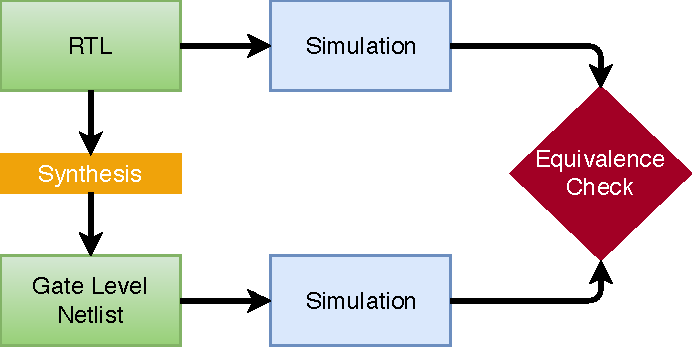
\includegraphics[width=0.7\textwidth]{Figures/Gate-level.pdf}
	\caption{Gate level design flow diagram.}
	\label{fig:gl}
\end{figure}

\subsection{Hardware-based Simulators}
\label{subsection:hardware}

As the name indicates, hardware-based simulators are a type of simulators that
rely on configurable hardware to do the digital circuit verification. When
compared with the software-based simulators, they have the advantage of being a
few orders of magnitude faster~\cite{tan:vhstas}. However they also have some
disadvantages: the hardware can be costly sometimes (depending on its
specifications) and it requires long compilation times, which makes them
needless for smaller designs. These simulators also require proprietary hardware
platforms to perform the desired simulations, with the hardware setup depending
on the platforms used, being different on each platform. As a result, these type
of simulators have a steep learning curve.

In this simulation type, the Verilog design is mapped onto a reconfigurable
piece of hardware with the same logical behavior as the netlist.  The simulation
is divided between the software simulator, which simulates all the Verilog code
that is not synthesizable, and the hardware accelerator, which simulates
everything that is synthesizable~\cite{khandelwal:gatelevel}. The design is then
run on the hardware, producing the simulation results. The results, like in a
Software-based simulator, must be checked in order to assess if the circuit is
working properly.

There are two variants of Hardware-based simulators: FPGA-based or
emulator-based. On one hand, the FPGA-based simulators, as the name indicates,
rely on FPGAs. A FPGA (Field Programmable Gate Array) is an integrated circuit
designed to be configured multiple times, according to the user needs. It
comprises an array of programmable logic blocks, memory elements, arithmetic
functions, etc.

The FPGA-based simulators follow the flow shown in Figure~\ref{fig:fpga}. The
original Verilog description of the code is transformed into an intermediate
representation, independent of the target platform. Here, the synthesizable
portions of the code are mapped into the FPGA, while the non synthesizable
portions (namely intendend for verification purposes) are run as software in the
host machine (software/hardware co-simulation). The simulator and the FPGA
interact with each other to produce the results.

\begin{figure}[!htb]
	\centering
	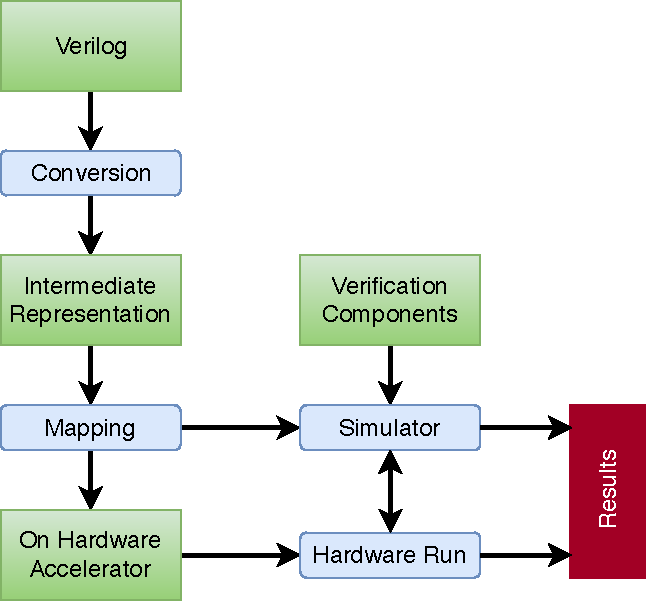
\includegraphics[width=0.7\textwidth]{Figures/FPGAsim.pdf}
	\caption{FPGA-based simulation flow~\cite{khandelwal:gatelevel}.}
	\label{fig:fpga}
\end{figure}

On the other hand, Emulator-based simulators rely on emulators to run their
simulations. An emulator is a specialized piece of hardware, that is , an
Application Specific Circuit (ASIC) that, when compared to a FPGA offers limited
reconfigurability, but with the advantage of a higher simulation speed. Even
though, the FPGA can run the actual circuit which in many cases superseeds
emulators in performance despite the lower clock frequency.

This type of simulation offers the possibility of testing software on the
developed design before having it implemented on chip, in a way that the
software application runs exactly as it would on the real chip in a real
circuit. It also offers the possibility for testing more complex programs, that
would take large amounts of time (sometimes even days) to run on other types of
simulators (like the software-based ones).

The simulation flow for this type of simulators has some similarities with the
FPGA-based simulators. In this case, as shown in Figure~\ref{fig:emulator}, the
Verilog code is converted into an intermediate representation, that will the be
mapped into the emulator. The code to be mapped must include only code that can
be implemented into the emulator. This means that the non synthesizable code
must be separated, being included in the software application. Both the software
and hardware platform interact with each other to produce the results.

\begin{figure}[!htb]
	\centering
	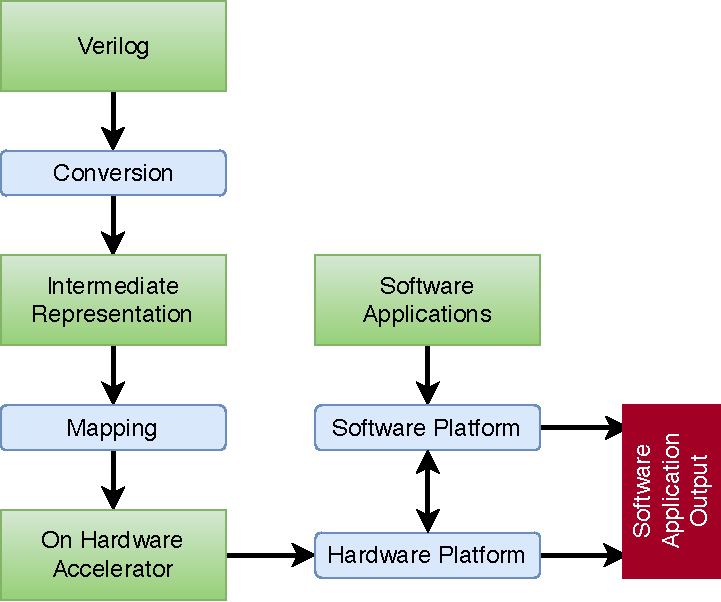
\includegraphics[width=0.7\textwidth]{Figures/Emulatorsim.pdf}
	\caption{Emulator-based simulation flow~\cite{khandelwal:gatelevel}.}
	\label{fig:emulator}
\end{figure}

\section{Cycle-Accurate Simulators}
\label{section:cycle}

Cycle-Accurate simulators are another important category of HDL
simulators. Instead of taking events sequentially, propagating them through the
circuit until it reaches a steady state, like the event-driven simulators, this
type of simulators evaluate each logic element of the circuit in a clock
cycle. They do this evaluation for each clock cycle, without taking into
consideration the propagation times and delays within the
cycle~\cite{khandelwal:gatelevel}.

As a result, these simulators are considerably faster than the event-driven
ones. However, they provide incomplete information about the circuit, since they
do not evaluate the delays and propagation times when evaluating each clock
cycle. So, if a circuit has timing problems, a cycle-accurate simulator will not
be able to notice them, making necessary the use of an even-driven simulator at
some stage to evaluate the existence of timing problems. All these
characteristics make the cycle-accurate simulators best suited for large circuit
simulation, like CPUs, when simulation speed is an important factor.

Most cycle-accurate simulators use a 2-state model (0 or 1) to calculate the
values of the signals through the circuit. A typical event-driven simulator uses
a more complex model, with more states (adding states like undefined, unknown or
high-impedance)~\cite{bennett:verilator}. This means that cycle-accurate
simulators have to make assumptions when the signals may have a value different
from 0 or 1 (for example, a signal that was uninitialized). While this speeds up
the simulation process, it also might be prone to produce wrong results.

From all the cycle-accurate simulators available, the most used one is probably
Verilator. Verilator is an open source simulator that compiles synthesizable
Verilog RTL, generating cycle accurate C++ and SystemC models. For each circuit, Verilator compiles a different model. These models are
then linked to a test bench, being executed in order to generate the
simulation. Verilator does not only translate Verilog code to C++ or
SystemC. Instead, it compiles the code into a much faster optimized and
thread-partitioned model, which is in turn wrapped inside a C++/SystemC
module~\cite{veripool:verilator}.

\section{Performance Comparison}
\label{section:performance}

When comparing event-driven and cycle-accurate simulators, not only their
working principles differ, but also their performance. Event-driven simulators
are typically slower than cycle-accurate simulators. This happens because the
algorithms used are more complex in event-driven simulators, having to implement
event scheduling and timing evaluation. The events are taken sequentially, being
propagated through the circuit until it reaches a steady state. New events
resultant from the output changes are added, meaning that the same element might
be evaluated multiple times during the same time step due to the feedback from
some signals. This whole process requires a considerable amount of time (and
computational power), being the main reason behind the lower speed of
event-driven simulators, when compared with cycle-accurate simulators.

The cycle-accurate simulators are typically the fastest type of simulators. This
happens because the simulation algorithm is simpler, evaluating each logic
element of the circuit in a clock cycle only once. They do this evaluation for
each clock cycle, without taking into consideration the propagation times and
delays within the cycle. There are also some simplifications that help improving
the simulation speed, like the use of a 2-state model (0 or 1) to calculate the
values of the signals through the circuit, instead of a model with multiple
states~\cite{bennett:verilator}.

In Figure~\ref{fig:performance} a graphic comparing the performance of the most
popular HDL simulators available in the market~\cite{verilator:benchmarks} is
shown. To run these benchmarks, a slightly modified model of the Motorolla M68K
processor was used. All the simulators shown were run in a general purpose
computer with an AMD Phenom 9500 2.2GHz processor, DDR2 667 Memory and running
the SuSE 11.1 operating system. The benchmark measures the number of cycles that
a simulator can run in a fixed amount of time, so a higher result means that
the simulator has a better performance.

From the analysis of the benchmark results, it can be concluded that Verilator
is considerably faster than the other tested simulators, both in 32 and 64 bits
versions. Cadence NCSim is almost 2 times slower than Verilator, while Synopsis
VCS is 3.5 times slower. Icarus Verilog is the slowest simulator tested, being
almost 80 times slower than Verilator. The benchmark results shown should only
work as reference, given their limitations: the versions of the simulators used
are already outdated, the same happening with the hardware and operating systems
used in the general purpose computers. Also, this benchmark only evaluates the
performance in one model (Motorolla M68K processor), instead of using multiple
models in order to provide more accurate results.

\begin{figure}[!htb]
	\centering
	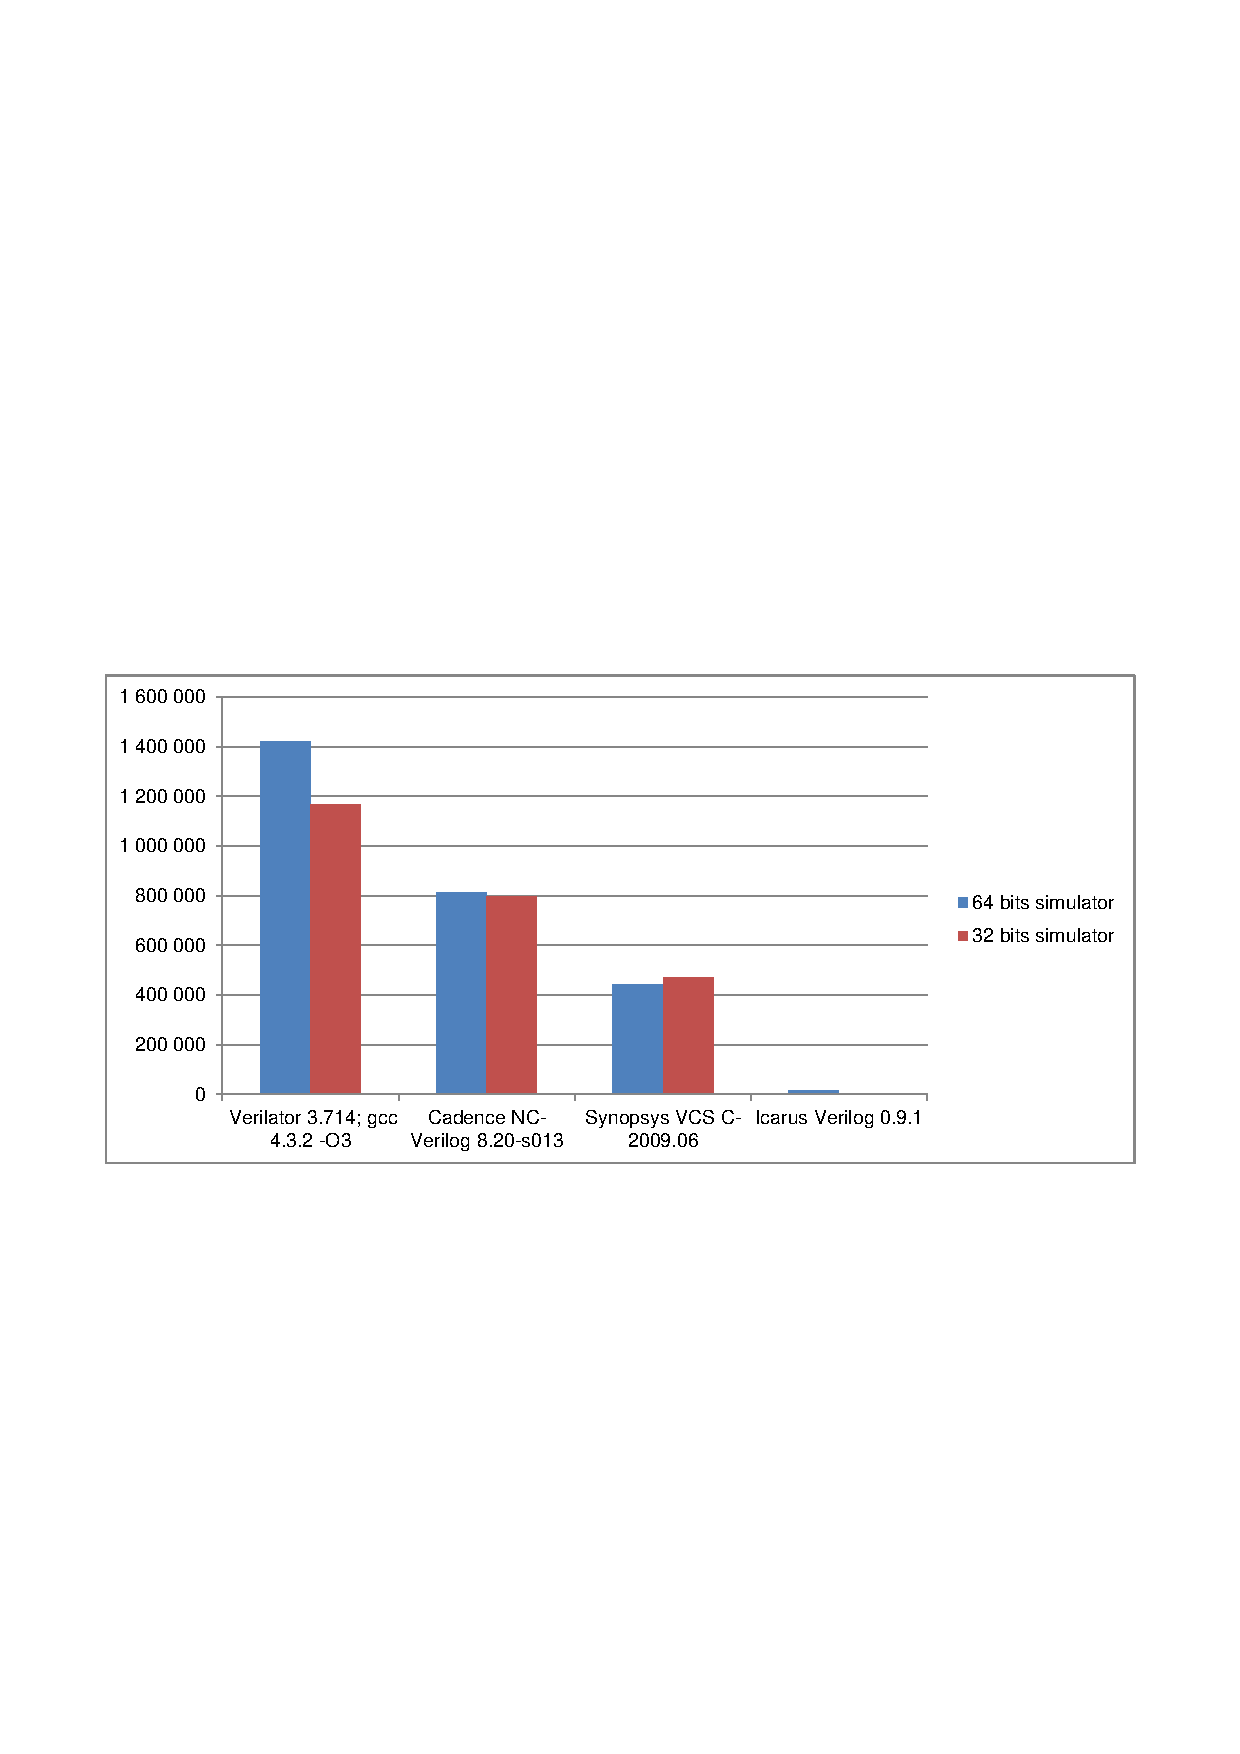
\includegraphics[trim=0 280 0 310 , clip, width=0.93\textwidth]{Figures/Performance.pdf}
	\caption{Benchmark results for different HDL simulators (higher means faster)~\cite{verilator:benchmarks}.}
	\label{fig:performance}
\end{figure}

The benchmark runs for the results shown in Figure~\ref{fig:performance} were
made in single-threaded mode. However, most commercial simulators (including the
ones analysed) support simulations in multi-threaded mode. This consists in
creating multiple threads for the different processes and distributing them
through multiple cores in a chip or even across multiple chips, that will be
executed in parallel. The threads are usually inter-dependent, so there should
be a synchronization process when transferring data between threads. This
process is time consuming, since different threads have different execution
times, requiring the faster threads to hold on until the slowest thread
finishes~\cite{tan:vhstas}.

Despite the concurrent nature of the Verilog statements, it isn't feasible to
parallelize the totality of the statements in a model, since the number of
statements is much greater than the amount of threads available, and also
because this would require a great amount of synchronization processes between
the different threads. Instead, the Verilog top-level code is divided in
multiple subsystems, with each one being simulated as a different thread.

The parallelization of HDL simulations is the solution found to achieve
considerable performance improvements in HDL simulators. This happens because
through the years the algorithms used in the simulators were optimized to such a
point where there were no further optimizations available, so the only viable
solution was to start using parallelization techniques.

%%  LocalWords:  parallelize
